\section{introduction}

In this chapter we'll have a brief showcase of the project, and where the modules
I've been working on are located within.

We'll start by describing the interface, and explain where the modules implemented
have been used in the goal of showcasing the seamlessness of the usage and 
how it eases up the complexity that exists in the back-end.

Some modules won't be showcased as they are not part of my implementation, and 
some won't be shown as they are kind of heavy on the back-end and impossible to
show unless you get a look at the code.

\section{Easy Truck In(ETI) in action}

Firstly we'll have a brief look at the East Truck In (ETI) interface, which is 
the main interface for the project. We'll specifically look into the user management
aspect.

\begin{figure}[!ht]
    \centering
    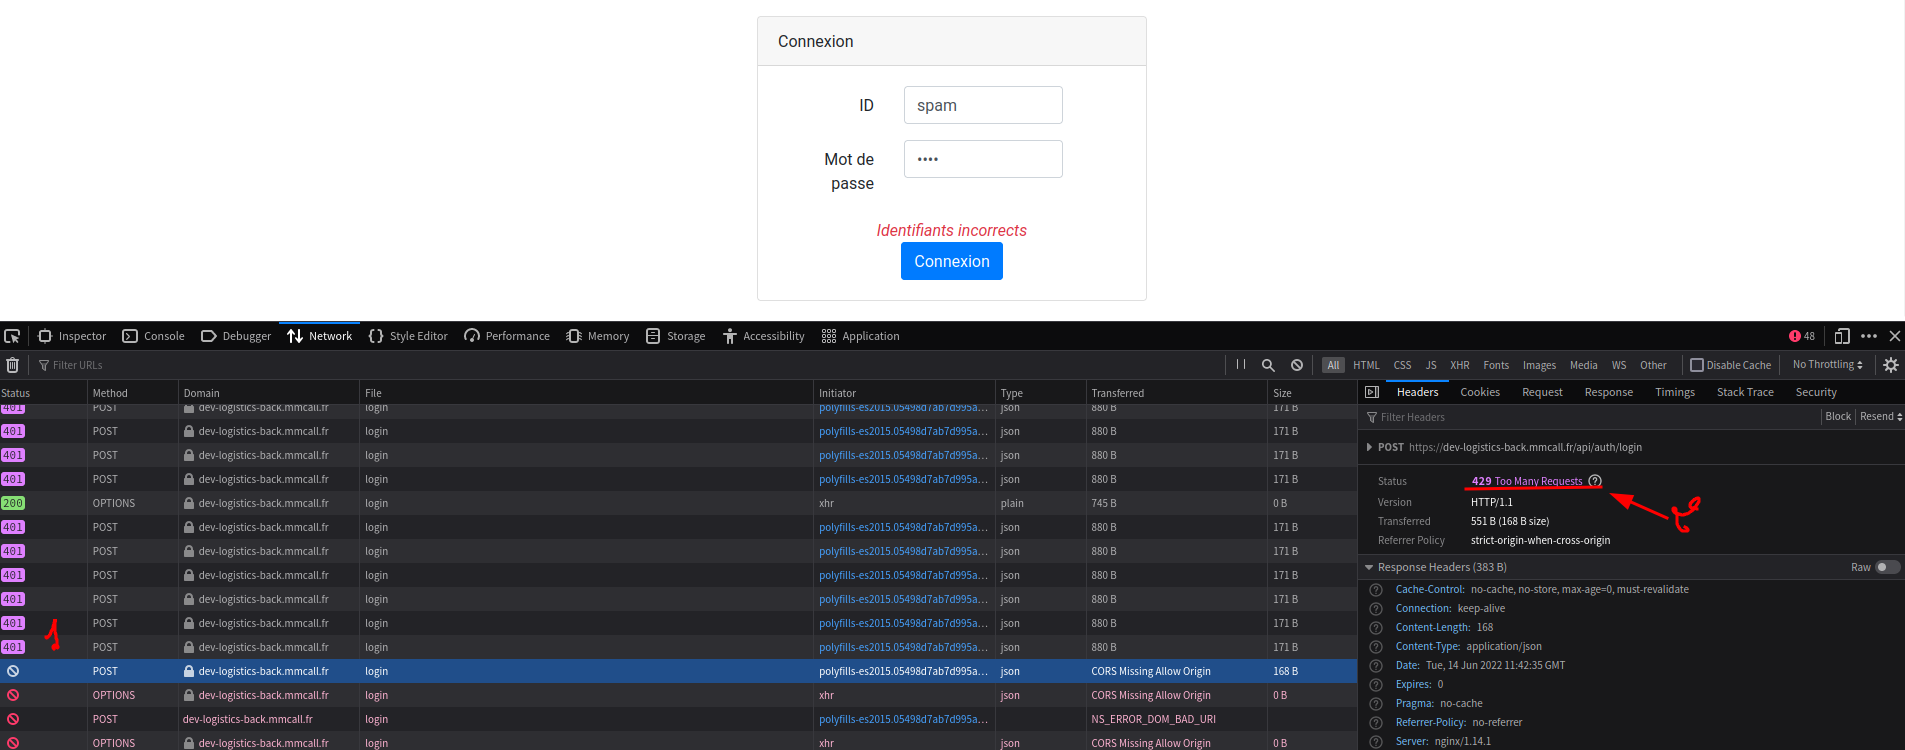
\includegraphics[width=\textwidth]{images/login too much attempts}
    \caption{\footnotesize{Login requests stopped after too much attempts}}
    \label{fig:login_req_ratelimit}
\end{figure}

In the figure \ref{fig:login_req_ratelimit} we can see that the login requests after a
certain number of attempts where the login was erroneous in purpose started getting
error 429, which is due to  the API rate limiter being triggered as we've discussed in
section \ref{subsec:ratelimiting}.

Next we'll take a look at the \ref{subsec:user_management} section, which is the
update of the user's profile, to make it easier to manage roles and have a overall easier
to use system.

\begin{figure}[!ht]
    \centering
    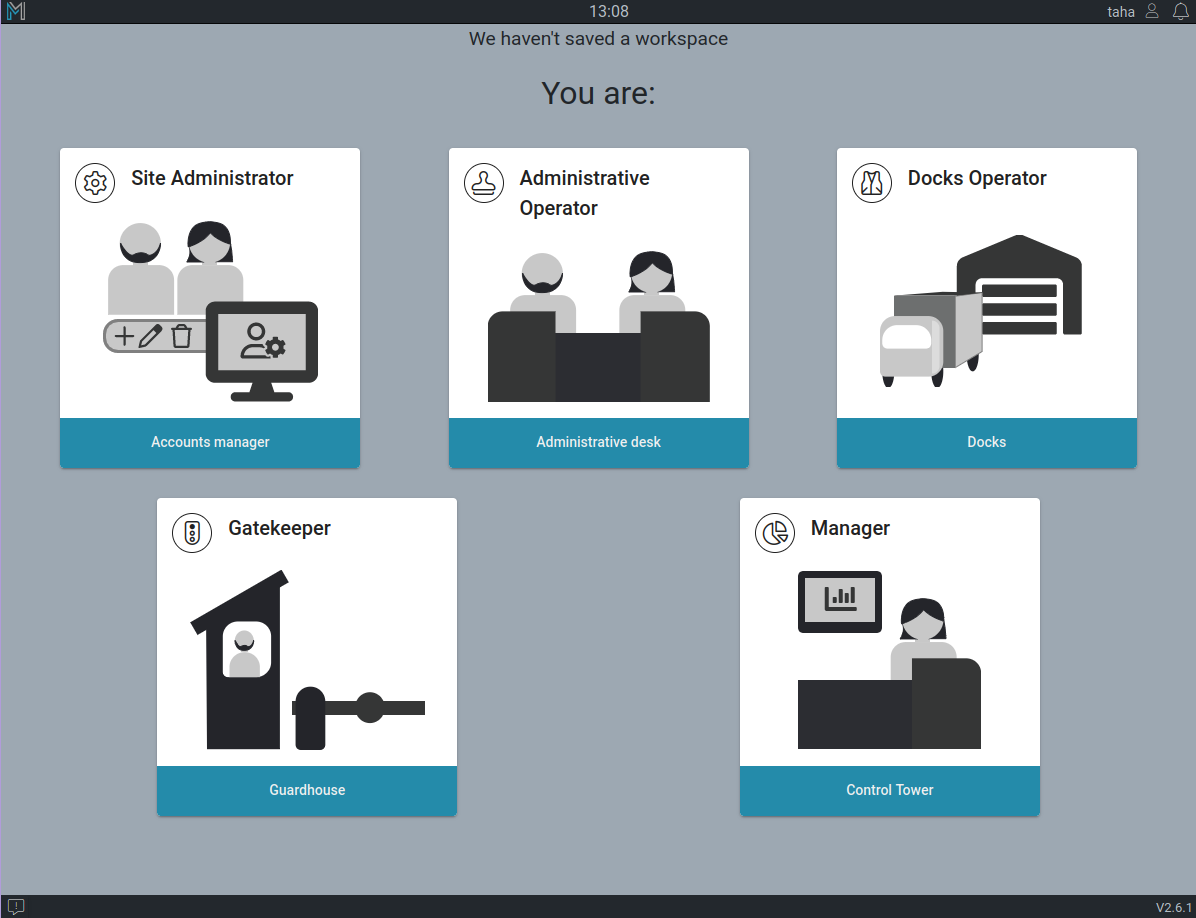
\includegraphics[width=0.49\textwidth]{images/user management}\hfill
    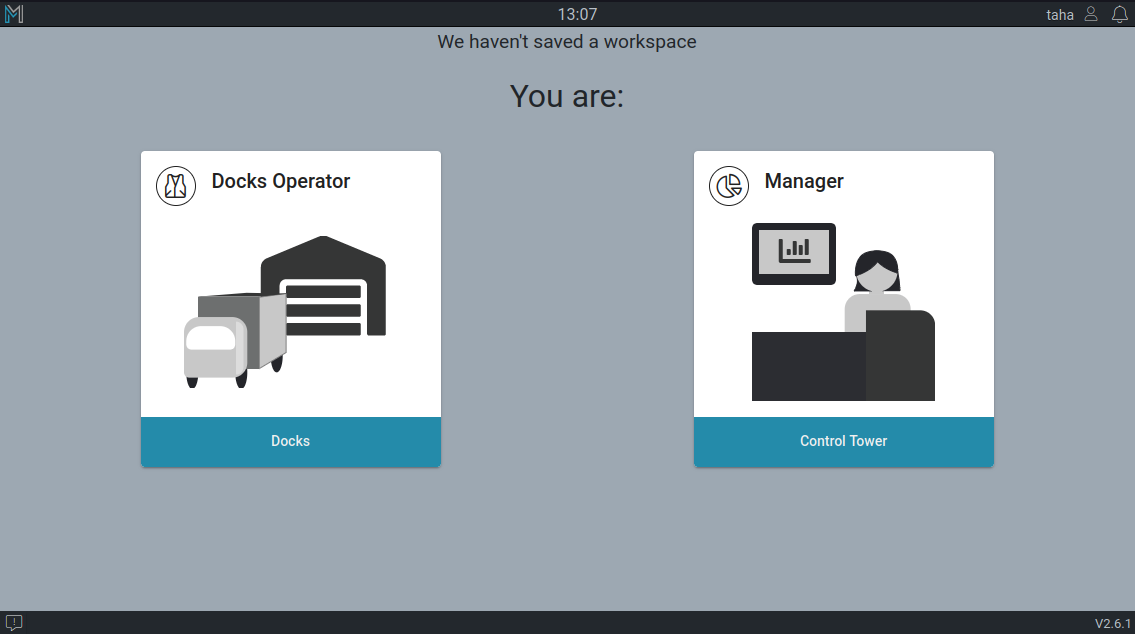
\includegraphics[width=0.49\textwidth]{images/userLessRoles}
    \caption{\footnotesize{ETI Main Page}}
    \label{fig:user_management_view}
\end{figure}

So the main view of the user management interface is the one in the figure
\ref{fig:user_management_view} which is a list of all workspaces available to the current
user, in my case I have access to all five workspaces.

So by removing a couple of workspaces from the current user from the database,
we can see that the user management interface is also updated and the workspaces
access change and that's due to the user management module we've implemented.

So here in 2nd figure \ref{fig:user_management_view}, we removed three workspaces from
the current user and we have access to only two workspaces.

So this access control is only doable by two types of users, the ones with the roles
of \textit{admin} which is a superuser and users who have the access role of
\textit{Account Manager} which is a user who can manage the accounts of other users.
From creating a new user to deleting a user, and they are related to the site.

\begin{figure}[!ht]
    \centering
    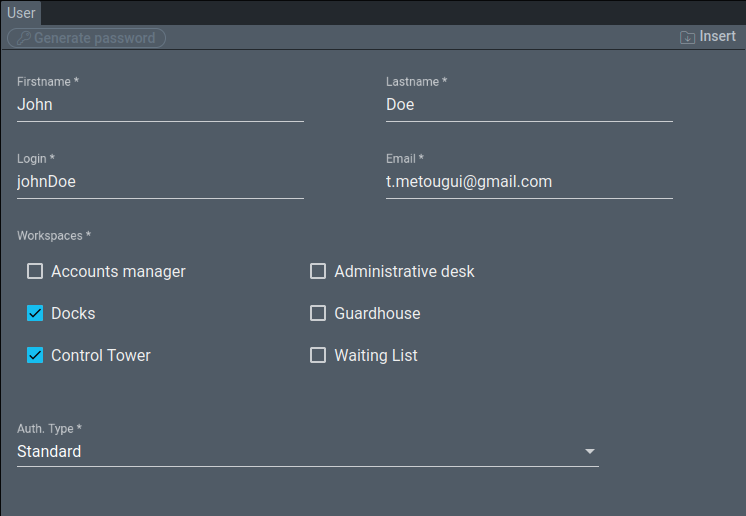
\includegraphics[width=0.49\textwidth]{images/insertingANewUser}
    \hfill
    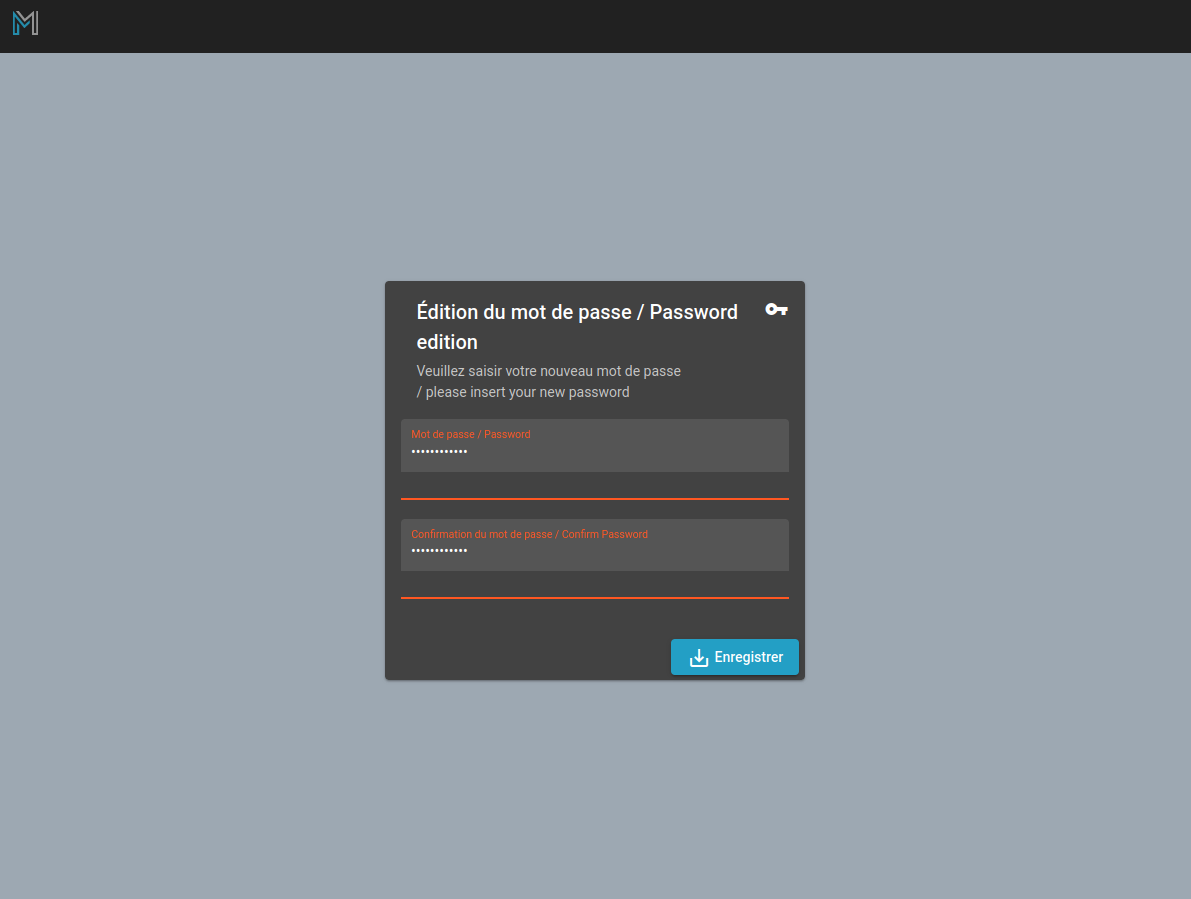
\includegraphics[width=0.49\textwidth]{images/password}
    \caption{\footnotesize{Adding a new user}}
    \label{fig:insert_user}
\end{figure}

The figure \ref{fig:insert_user} shows the part in account management where we can add
a new user to the system. Giving power to control his roles and workspaces.

\begin{figure}[!ht]
    \centering
    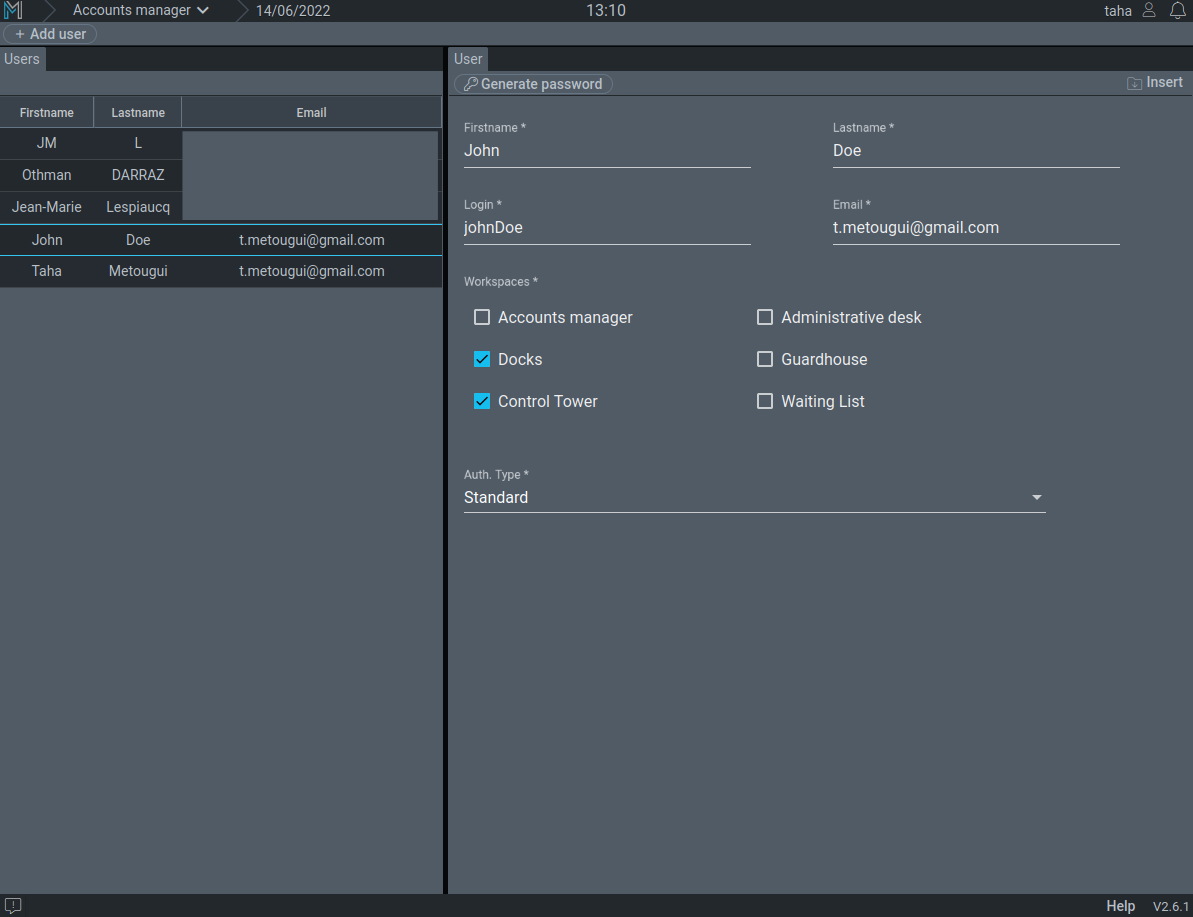
\includegraphics[width=\textwidth]{images/accManager}
    \caption{\footnotesize{Account Manager}}
    \label{fig:accManager}
\end{figure}

Once added the user is shown in the list of users, on the side of the page. As shown in 
figure \ref{fig:accManager} where we can see all the users that are in the site the 
current user is in.

Once user added, we get the possibility to create a new password for the user. By clicking
the generate password button, then a email is sent to the user and then you receive the
email in your inbox that redirects you to a page in 2nd figure \ref{fig:insert_user} where
it can be seen that the client gets invited to introduce their password.
Such a mechanism is put in place because the users can only be created by account managers.

As for the rest of the workspaces their business logic is mostly for the fleet management, 
and wasn't in the scope of my implementation except for creating roles for those workspaces
to be accessible.

\section{Conclusion}

To conclude, this was a showcase of the user management module and the API rate limiting
part, for the user management it was quite a clear and easy to use interface that hides
all the complexity of the data structures within and makes good use of the API callbacks.
For the API ratelimiting we've just shown the basic idea of log in attempts, and how it
got stopped once the limit was reached, and it's the same for API rate limiting on other
endpoints but just in a different number of possible calls.

For the rest of the contributions, specifically the Containeraization and deployment
it's just a pure infrastructure logic, and improvement. So couldn't really get a way
to showcase it in a simplified way and also it's not important for the end user to
get interacting with these points.
